\documentclass{beamer}
%[aspectratio=169]   \usepackage[czech]{babel}
\usepackage{apo-lecture-en}
\usepackage{pdfpages}
\usepackage{pdfcomment}
\usepackage{listings}

\subtitle{Lecture 11. x86 Architecture}
\author{Pavel Píša \phantom{xxxxxxxxx} Petr Štěpán \\ \small\texttt{pisa@fel.cvut.cz}\phantom{xxxx}\small\texttt{stepan@fel.cvut.cz}}
\begin{document}

\maketitle

\section{x86 History}

\begin{frame}
\frametitle{Processor -- CPU}
\begin{columns}[t,onlytextwidth]
\begin{column}{0.4\textwidth}
Basic features:
  \begin{itemize}
    \item data and address bus width
    \item number and size of internal registers
    \item control signal rate -- frequency
    \item instruction set
  \end{itemize}
\end{column}
\begin{column}{0.52\textwidth}  
   \begin{center}
   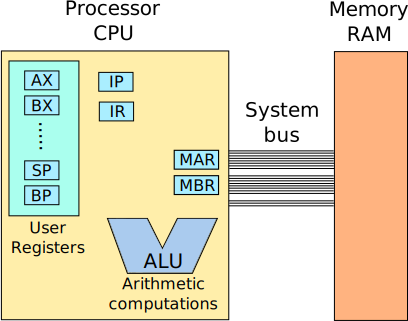
\includegraphics[width=0.9\textwidth]{cpu-en.pdf}
   \end{center}
\end{column}
\end{columns}
\end{frame}


\begin{frame}
\frametitle{x86/AMD64 -- History}
\begin{itemize}
\item x86 - CPU family, x is placeholder for x values - 0,1,2,3,4,5,6
\end{itemize}

\begin{columns}[t,onlytextwidth]
\begin{column}{0.48\textwidth}
\textbf{8086} -- R16 A20 (1978) the first IBM PC (8088 - 1979) \\
\textbf{80286} -- R16 A24 (1982) protected mode\\
\textbf{80386} -- R32 A32 (1985) paging\\
\textbf{80486} -- R32 A32 (1989) pipelining, FPU, cache\\
\textbf{80586} -- R32 A32 (1993) Pentium superscalar\\
\end{column}
\begin{column}{0.48\textwidth}  
\textbf{80686} -- R32 A36 (1995) Pentium Pro PAE, L2 cache, out-of-order \& speculative exec\\
\textbf{IA-64} -- R64 A52 (2001) Itanium 64-bit version\\
\textbf{AMD64} -- R64 A40 (2003) Athlonn 64-bit version from AMD\\
\textbf{Core2} -- R64 A36 (2006) Intel 64 EM64T, SSSE3, $\mu$op, virtualization
\end{column}
\end{columns}

\begin{itemize}
\item More detailed list -- \url{https://en.wikibooks.org/wiki/X86\_Assembly}
\end{itemize}

\end{frame}

\begin{frame}[shrink=1.2]
\frametitle{x86/AMD64 -- Registers}
\small
User/General Purpose Registers
\begin{itemize}
\item All registers are 64/32/16/8 bit for backward compatibility
\item integer registers for storing program values ​​\texttt{eax}, \texttt{ebx}, \texttt{ecx}, \texttt{edx}
\item specialized registers as memory pointers \texttt{esi}, \texttt{edi}, \texttt{ebp}
\item \texttt{esp} -- stack pointer - more details below
\item AMD64/EM64T adds 8 additional registers \texttt{r8}-\texttt{r15}, in the form of \texttt{r8b} lowest byte, \texttt{r8w} lowest word (16 bits), \texttt{r8d} -- lower 32 bits, \texttt{r8} -- 64 bit register
\end{itemize}
\begin{center}
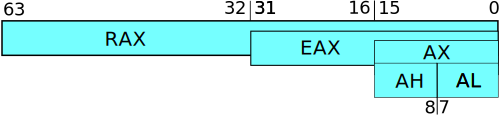
\includegraphics[width=0.5\textwidth]{registers.pdf}
\end{center}
Control and Status Registers
\begin{itemize}
\item \texttt{IP/EIP/RIP} -- instruction pointer -- points to the current executed instruction
\item \texttt{FLAGS/EFLAGS/RFLAGS} -- program status word/flags registers
\end{itemize}

\end{frame}



\begin{frame}
\frametitle{x86/AMD64 -- FLAGS Register}
RFLAGS register
\begin{center}
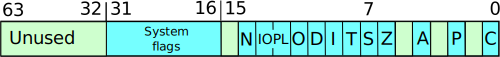
\includegraphics[width=0.65\textwidth]{flags-en.pdf}
\end{center}
\begin{columns}[t,onlytextwidth]
\begin{column}{0.5\textwidth}
C -- Carry flag\\
P -- Parity flag\\
Z -- Zero flag\\
S -- Sign flag\\
O -- Overflow flag\\
A -- Auxiliary flag (BCD)
\end{column}
\begin{column}{0.5\textwidth}  
I -- Interrupt enable\\
T -- Trap flag\\
IOPL -- I/O privilege level\\
System Flags:
\begin{itemize}
\item VM -- Virtual 8086 Mode
\item VIF -- Virtual Interrupt Flag
\item VIP -- Virtual Interrupt Pending
\end{itemize}
\end{column}
\end{columns}
\end{frame}

\begin{frame}
\frametitle{x86/AMD64 -- Operating Modes}
FLAGS register 
\begin{itemize}
  \item Only two protection rings/modes used -- the base of the hardware protections
  \begin{itemize}
    \item CPL0\footnote{Current privilege level} =  privileged (system) mode
    \begin{itemize}
      \item processor can access hardware (I/O ports), manipulate paging state etc. 
    \end{itemize}
    \item CPL3 = user (application) mode
    \begin{itemize}
      \item privileged operations are not permitted
    \end{itemize}
  \end{itemize}
  \item Privileged operations
  \begin{itemize}
    \item manipulation with system/core state (halt, reset, Interrupt Enable/Disable, whole Flags modifications, MMU registers changes and control instructions) 
    \item I/O port access instructions (in, out)
  \end{itemize}

  \item Switching between modes and privileges
  \begin{itemize}
    \item The old 16 real mode after system reset, start at address 0xffff:0000
    \item Complex sequence to switch into 64-bit mode at CPL0 (system)
    \item Switch to user (CPL3) mode -- Flags registers change (popf or reti)
    \item Switch to system (CPL0) mode -- only by interrupt, including synchronous by int instruction
  \end{itemize}
\end{itemize}
\end{frame}


\section{x86 -- Instruction Set}

\begin{frame}
\frametitle{x86/AMD64 Instructions}
Data transfers register to register and immediate to register \\
(Two different syntaxes are commonly used for x86 assembler code.)\\

\begin{tabular}{ l l }
\textbf{AT\&T} & \textbf{Intel}\\
\texttt{movq} source 64b, dest &	\texttt{mov} dest, source\\
\texttt{movl} source 32b, dest &\\
\texttt{movw} source 16b, dest &\\
\texttt{movb} source 8b, dest &\\
registers  &\\
\texttt{\%ax}	& only \texttt{ax}\\
immediate \$, hex 0x & number, hex postfix h\\
&\\
\texttt{movl \$0xff, \%ebx} & \texttt{mov ebx, 0ffh}\\
\end{tabular}

If the source width is n-ener than destination, two variants exists:
\begin{itemize}
 \item movsX -- sign extension, the MSB is expanded to additional bits
 \item movzX -- zero extension, the destination additional bits are zeroed
\end{itemize}
 
\end{frame}


\begin{frame}
\frametitle{x86/AMD64 -- Instructions}
Data transfers to/from memory (memory pointers / register indirect)\\
\begin{tabular}{ l l}
AT\&T & Intel \\
\texttt{movl (\%ecx),\%eax} & \texttt{mov eax, [ecx]}\\
\texttt{movl 3(\%ebx), \%eax} & \texttt{mov eax, [ebx+3]} \\
\texttt{movl (\%ebx, \%ecx, 0x2), \%eax} & \texttt{mov eax, [ebx+ecx*2h]} \\
\texttt{movl -0x20(\%ebx, \%ecx, 0x4), \%eax} & \texttt{mov eax, [ebx+ecx*4h-20h]} \\
\end{tabular}

\begin{itemize}
\item effective address has 4 components: \emph{base+index*scale+offset}
\item the \emph{scale} possible values are 1,2,4,8
\item directly maps to array of structures access: \emph{base} points to array start, \emph{index*scale} specifies which entry/index and \emph{offset}, which structure field is accessed.
\item it is not required that all four address components are used each time
\end{itemize}
\end{frame}


\begin{frame}
\frametitle{x86/AMD64 -- Repeat Prefix and String Operations}
Instructions for string/bloc operations  - \texttt{REP} prefix for repeat over array
\begin{itemize}
\item repeat while \texttt{ecx>0}:
\begin{itemize}
\item \texttt{operations (\%esi), (\%edi)}
\item \texttt{esi += d*operand\_size}
\item \texttt{edi += d*operand\_size}
\item \texttt{ecx - -}
\end{itemize}
\item string operations \texttt{movs, cmps, lods, stos, scas, ins, outs}
\item \texttt{d} - direction specification values +1, or -1
\item \texttt{REP} repeat \texttt{ecx} specified times
\item \texttt{REPE/REPNE} repeat max \texttt{ecx} times while condition is true
  \begin{itemize}
  \item operation \texttt{cmps} stops if there is/not differece between \texttt{[edi]} and \texttt{[esi]} memory locations
  \item operation \texttt{scas} stops if there is/not differece between \texttt{[edi]} and \texttt{eax} register value
  \end{itemize}
\end{itemize}

\end{frame}


\begin{frame}[fragile]
\frametitle{x86/AMD64 -- Repeat Example -- Fill Array}
Set each array element to the -1 value:
\begin{minted}[fontsize=\footnotesize]{c}
int array[128];
for (int i=0; i<128; i++) {
  array[i]=-1;
}
\end{minted}
translated:
\begin{minted}[fontsize=\footnotesize]{gas}
mov   array, %edi  ; Set edi register to points to the array start
mov   $128,  %ecx  ; Setup number of repetitions
mov   $-1,   %eax  ; Set the value to be stored
rep   stosd        ; Fill the whole array
\end{minted}
\end{frame}


\begin{frame}[fragile]
\frametitle{x86/AMD64 -- Zero Terminated String Length}

Find end of the zero terminated string:
\begin{minted}[fontsize=\footnotesize]{c}
char str[128];
int i;
for (i=0; i<128; i++) {
  if (str[i]==0) 
    break;
}
\end{minted}
translated:
\begin{minted}[fontsize=\footnotesize]{gas}
mov   str,  %edi  ; Set EDI to point to start of the string
mov   $128, %ecx  ; Setup maximal number of repetitions
mov   $0,   %eax  ; Set register for the search value (0)
repne scasb       ; Scan the str until 0 is located
\end{minted}

\end{frame}



\begin{frame}
\frametitle{x86/AMD64 -- Arithmetic Operations}
Arithmetic -- AT\&T syntax

the \textit{X} placeholder for next operatins allowed values are \texttt{b}, \texttt{w}, \texttt{l}, \texttt{q}\\
The source (\textit{src}) is applied through specified operation to the value at destination (\textit{dst}) and result is stored to the same destination
\begin{tabular}{ l l}
\texttt{addq  \$0x05,\%rax} & rax = rax + 5\\
\texttt{subl  -4(\%ebp), \%eax} &  eax = eax -- mem(ebp-4)\\
\texttt{subl  \%eax, -4(\%ebp)} & mem(ebp-4) = mem(ebp-4)-eax\\
\texttt{and\textit{X}} \textit{src}, \textit{dst} & bitwise and\\
\texttt{or\textit{X}}  \textit{src}, \textit{dst} & bitwise or\\
\texttt{xor\textit{X}} \textit{src}, \textit{dst} & bitwise xor (fast register clear)\\
\texttt{mul\textit{X}} \textit{multiplier} & multily \texttt{eax} by unsigned value  $\rightarrow$  \texttt{edx:eax}\\
\texttt{div\textit{X}} \textit{divisor} & divide \texttt{edx:eax} by unsigned value\\
\texttt{imul\textit{X}} \textit{multiplier} & multiply \texttt{eax} by signed value  $\rightarrow$ \texttt{edx:eax}\\
\texttt{idiv\textit{X}} \textit{divisor} & divide \texttt{edx:eax} by signed value\\
\end{tabular}
\end{frame}

\begin{frame}
\frametitle{x86/AMD64 -- Single Operand Functions}
Arithmetic with single operand -- AT\&T syntax
\begin{tabular}{ l l}
operation &\\
\texttt{incl            \%eax} &              eax = eax + 1\\
\texttt{decw            (\%ebx)} &                 mem(ebx) = mem(ebx)-1\\
\texttt{shlb            \$3, \%al} &                al = al$<<$3\\
\texttt{shrb            \$1, \%bl} &                bl=11000000, po bl=01100000\\
\texttt{sarb            \$1, \%bl} &                bl=11000000, po bl=11100000\\
\texttt{ror\textit{X}, rol\textit{X}} & rotate left/right by n bits.  \\
\texttt{rcr\textit{X}, rcl\textit{X}} & rotate left/right by n bits with C -- carry flag\\
\end{tabular}
\end{frame}


\begin{frame}
\frametitle{x86/AMD64 -- Flow Control}
Conditional branches\\
\begin{tabular}{ l l}
\texttt{test    a1, a2} &  tmp = a1 AND a2, Z tmp=0, C tmp<0\\
\texttt{cmp     a1, a2} &  tmp = a1-a2, Z tmp=0, C tmp<0\\
\end{tabular}

next jump/branch instructions can be used then
\begin{tabular}{ l l}
\texttt{jmp \textit{taget}} & unconditional jump, equivalent to \texttt{\%eip=taget}\\
\texttt{je  \textit{taget}} & jmp equal -- jump when equal (Z=1)\\
\texttt{jne \textit{taget}} & jmp not equal -- jump when not equal (Z=0)\\
\texttt{jg/ja \textit{taget}} & jmp greater/above -- jump when a1 > a2 (sign/unsig)\\
\texttt{jge/jae \textit{taget}} & jump if a1 >= a2 (sign/unsig)\\
\texttt{jl/jb \textit{taget}} & jmp less/below -- jump when a1 < a2 (sign/unsig)\\
\texttt{jle/jbe \textit{taget}} & jump if a1 <= a2 (sign/unsig)\\
\texttt{jz/jnz \textit{taget}} & jump if Z=1/0\\
\texttt{jo/jno \textit{taget}}& jump when O (overflow) = 1/0\\
\end{tabular}
\end{frame}

\begin{frame}
\frametitle{Quiz}
Is the difference for program sizes for CISC (x86) and RISC (RISC-V)?
\begin{itemize}
\item[A] no difference, approximately the same
\item[B] CISC programs are longer
\item[C] RISC programs are longer
\end{itemize}
\end{frame}


\begin{frame}[fragile]
\frametitle{Comparison of CISC vs. RISC Program}
CISC programs are usually shorter if compressed (16-bit) encoding is not used on RISC side:
\begin{minted}[fontsize=\footnotesize]{gas}
incl 10(%ecx)   -      lw   t2, 10(t1)
                       addi t2, t2, 1
                       sw   t2, 10(t1)

rep movs        - l1:  lw   t3, 0(t1) 
                       sw   t3, 0(t2)
                       addi t1, t1, 4
                       addi t2, t2, 4
                       addi t4, t4, -1
                       bne  t4, zero, l1 
\end{minted}
On the other hand, larger number of GPR registers and return address storage in the register instead on the stack leads to lower number of accesses to memory which is advantage even if memory is cached.
\end{frame}

\begin{frame}
\frametitle{Quiz}
Are CISC (x86) programs faster than RISC (RISC V) programs?
\begin{itemize}
\item[A] Yes
\item[B] No
\item[C] It depends
\item[D] Every today superscalar high performance architecture uses RISC style instructions processing internally
\end{itemize}

\end{frame}



\begin{frame}
\frametitle{Stack for Calls, Arguments, Save and Local Variables}

\begin{columns}
\begin{column}{0.45\textwidth}
\small
Stack:
\begin{itemize}
\item LIFO data structure
\end{itemize}

Implementation:
\begin{itemize}
\item dedicated \textit{SP} register - points to the stack top
\item before every \texttt{push} (data save) operation, \textit{SP} is decremented by operand size, for every \texttt{pop} (register restore) operation, the \textit{SP} is incremented by same size
\end{itemize}
\begin{tabular}{ l l}
\texttt{pushl \%eax} &  save \texttt{eax} onto stack top\\
\texttt{popw \%bx}   &  restore 16-bit \texttt{bx} register \\
                     &  and icrements \textit{SP} by 2\\
\texttt{pushf/popf}  &  save/restore EFLAGS\\
                     &  register \\
\texttt{pusha/popa}  &  save/restore all\\
                     &  user registers\\
\end{tabular}
\end{column}

\begin{column}{0.55\textwidth}  
\small
\begin{itemize}
\item \texttt{push} operation saves data into stack
\begin{itemize}
\item \texttt{sub \$size, sp}
\item \texttt{mov \%eax, 0(sp)}
\end{itemize}
\item \texttt{pop} restores data from the stack
\begin{itemize}
\item \texttt{mov 0(sp), \%eax}
\item \texttt{add \$size, sp}
\end{itemize}
\item it is possible to access stack with offsets same as for RISC-V:
\begin{itemize}
\item \texttt{sub \$16, sp}
\item \texttt{mov \%eax, 0(sp)}
\item \texttt{mov \%ebx, 4(sp)}
\item \texttt{mov \%ecx, 8(sp)}
\item \texttt{mov \%edx, 12(sp)}
\end{itemize}
\end{itemize}
\end{column}
\end{columns}
\end{frame}


\begin{frame}[fragile]
\frametitle{Quiz}

Which program is executed faster by the superscalar architecture implementation:
\begin{columns}
\begin{column}{0.45\textwidth}
A
\begin{minted}[fontsize=\footnotesize]{gas}
push %eax
push %ebx
push %ecx
push %edx
\end{minted}
\end{column}
\hfill
\begin{column}{0.45\textwidth}  
B
\begin{minted}[fontsize=\footnotesize]{gas}
sub $16, sp
mov %eax, 0(sp)
mov %ebx, 4(sp)
mov %ecx, 8(sp)
mov %edx, 12(sp)
\end{minted}
\end{column}
\end{columns}

\begin{itemize}
\item[A] Both take similar time
\item[B] A is faster to execute than B
\item[C] B is faster to execute than A
\item[D] Cannot be determined
\end{itemize}
\end{frame}

\begin{frame}
\frametitle{x86 Function Calling Convetion for 32-bit "cdecl"}

\begin{itemize}
\item The caller saves all parameters on the stack
\item The order of saving on the stack is from the last parameter to the first
\end{itemize}

\bigskip

function calling\\
\begin{tabular}{ l l}
\texttt{call adr} &         equivalent to \texttt{push \%eip}, \texttt{jmp adr}\\
\end{tabular}\\
return from the function\\
\begin{tabular}{ l l}
\texttt{ret} &              equivalent to \texttt{pop \%eip}\\
\end{tabular}\\
\bigskip

\begin{itemize}
\item The function return/result value will be stored in the \texttt{eax} register.
\item The registers \texttt{ebp}, \texttt{ebx}, \texttt{esi}, \texttt{edi} must be preserved by the function. If the function has use for them, the original value must be saved on the stack.
\end{itemize}

\end{frame}


\begin{frame}[fragile]
\frametitle{x86 Function Calling -- Function Stack Frame}
The \texttt{ebp} register points to the stack where previous \texttt{ebp} of caller function was stored\\
\bigskip
Function prologue example
\begin{minted}[fontsize=\footnotesize]{gas}
push  %ebp        ; Caller EBP value is stored to stack
mov   %esp, %ebp  ; Remember actual stack position in EBP
sub   $12, %esp   ; Reserve 12 bytes for local variables,
                  ; registers save and or call arguemnts
\end{minted}

The first local variable or save would be at  \texttt{-4(\%ebp)}, next \texttt{-8(\%ebp)}\\
The first argument at address \texttt{8(\%ebp)}, next \texttt{12(\%ebp)}

Function epilogue -- finalization:
\begin{minted}[fontsize=\footnotesize]{gas}
mov   %ebp, %esp  ; Restore stack top to the original position
pop   %ebp        ; Restore original EBP register value
ret               ; Return from the function
\end{minted}

The cobined instruction for restore stack state at return:
\texttt{leave} is equivalent for:
\begin{minted}[fontsize=\footnotesize]{gas}
mov   %ebp, %esp 
pop   %ebp
\end{minted}

\end{frame}

\begin{frame}[fragile]
\frametitle{x86 Function Calling -- Example}

\begin{columns}
\begin{column}{0.35\textwidth}
Function calling:

\begin{minted}[fontsize=\footnotesize]{c}
t = addfour(1, 2, 3, 4);
\end{minted}

Compiled x86 machine code
\begin{minted}[fontsize=\footnotesize]{gas}
push $4
push $3
push $2
push $1
call 10e2 <addfour>
add $0x10, %esp
\end{minted}
\end{column}


\begin{column}{0.35\textwidth}  
Function prologue
\begin{minted}[fontsize=\footnotesize]{gas}
push %ebp
mov  %esp, %ebp
push %ebx
sub  $0x10, %esp
\end{minted}

Access to local variables:
\begin{minted}[fontsize=\footnotesize]{gas}
mov %eax, -4(ebp)
\end{minted}

The first and the second argument access:
\begin{minted}[fontsize=\footnotesize]{gas}
mov 0x8(ebp), %edx
mov 0xc(ebp), %eax
\end{minted}

Function epilogue -- finalization:
\begin{minted}[fontsize=\footnotesize]{gas}
leave
ret
\end{minted}
\end{column}

\begin{column}{0.3\textwidth}  
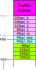
\includegraphics[width=0.95\textwidth]{fnc_frame-en.pdf}
\end{column}

\end{columns}
\end{frame}


\begin{frame}
\frametitle{AMD64 Function Calling Convention -- ELF/Linux}

\begin{itemize}
\item Up to 6 integer arguments are passed in \texttt{rdi}, \texttt{rsi}, \texttt{rdx}, \texttt{rcx}, \texttt{r8}, \texttt{r9} and or up to 8 floating point arguments are passed in \texttt{zmm0}-\texttt{7}
\item The rest of the arguments is passed by stack. The \texttt{al} is required to hold number of \texttt{zmm\textit{X}} used for variadic functions or functions without prototype calls.
\end{itemize}

\medskip

\begin{itemize}
\item The function's return value will be stored in the \texttt{rax} and \texttt{rdx} registers.
\item The \texttt{rbp}, \texttt{rbx}, \texttt{r12}-\texttt{r15} registers must be preserved by the function. If the function wants to use them, the original value must be saved to the stack.
\item Red Zone -- a zone 128 bytes from the \texttt{rsp} pointer that must not be changed by the interrupt handler. This zone allows this memory to be used for temporary variables without moving the rsp pointer.
Of course, calling the function changes this zone.
\end{itemize}

\end{frame}



\begin{frame}
\frametitle{Stack Purposes}

Stack:
\begin{itemize}
  \item parameters for the function (currect and called)
  \item return address, next instruction to continue after function call is finshed
  \item local variables of the function
  \begin{itemize}
     \item the stack is usually small
     \item limited size of local variables
     \item be careful with recursion - it is better to avoid recursion
  \end{itemize}
\end{itemize}

\end{frame}



\begin{frame}[fragile]
\frametitle{Quiz}

Consider program:
\begin{columns}
\begin{column}{0.45\textwidth}
\begin{lstlisting}[language={C},columns=flexible]
int factorial(int x) {
  int y;
  if (x<=1) {
    return 1;
  } else {
    y = factorial(x-1)
    return y*x;
  }
}
\end{lstlisting}
\end{column}
\hfill
\begin{column}{0.45\textwidth}  
\begin{lstlisting}[language={C},columns=flexible]
int i;
int main() {
  i=10;
  i=factorial(i);
  return i;
}
\end{lstlisting}
\end{column}
\end{columns}

Where is allocated space for \texttt{i} local variable?
\begin{itemize}
\item[A] On stack for both RISC-V and x86.
\item[B] Allocated from heap on RISC-V and on the stack for x86.
\item[C] In the \texttt{.data} or \texttt{.bss} section for both RISC-V and x86.
\item[D] In the register for both RISC-V and x86.
\end{itemize}
\end{frame}


\begin{frame}[fragile]
\frametitle{Quiz}

Consider program:
\begin{columns}
\begin{column}{0.45\textwidth}
\begin{lstlisting}[language={C},columns=flexible]
int factorial(int x) {
  int y;
  if (x<=1) {
    return 1;
  } else {
    y = factorial(x-1)
    return y*x;
  }
}
\end{lstlisting}
\end{column}
\hfill
\begin{column}{0.45\textwidth}  
\begin{lstlisting}[language={C},columns=flexible]
int i;
int main() {
  i=10;
  i=factorial(i);
  return i;
}
\end{lstlisting}
\end{column}
\end{columns}

Location for \texttt{y} variable when compiled without optimization?
\begin{itemize}
\item[A] On the stack or in the register for both RISC-V and x86.
\item[B] Dynamically allocates on heap for both RISC-V and x86
\item[C] In the \texttt{.data} or \texttt{.bss} section for both RISC-V and x86.
\item[D] cannot be determined for RISC-V neither x86.
\end{itemize}
\end{frame}

\begin{frame}[fragile,shrink=10]
\frametitle{Quiz}

Consider program:
\begin{columns}
\begin{column}{0.45\textwidth}
\begin{lstlisting}[language={C},columns=flexible]
int factorial(int x) {
  int y;
  if (x<=1) {
    return 1;
  } else {
    y = factorial(x-1)
    return y*x;
  }
}
\end{lstlisting}
\end{column}
\hfill
\begin{column}{0.45\textwidth}  
\begin{lstlisting}[language={C},columns=flexible]
int i;
int main() {
  i=10;
  i=factorial(i);
  return i;
}
\end{lstlisting}
\end{column}
\end{columns}

Location of \texttt{x} variable for compilation without optimization?
\begin{itemize}
\item[A] RISC-V and x86: on stack
\item[B] RISC-V: in register; x86: on stack
\item[C] RISC-V: in register and then on stack; x86: on stack
\item[D] RISC-V: on stack; x86: in register
\item[E] RISC-V: on stack; x86: in register and then on stack
\end{itemize}
\end{frame}

\begin{frame}[fragile,shrink=10]
\frametitle{Quiz}

Consider program:
\begin{columns}
\begin{column}{0.45\textwidth}
\begin{lstlisting}[language={C},columns=flexible]
int factorial(int x) {
  int y;
  if (x<=1) {
    return 1;
  } else {
    y = factorial(x-1)
    return y*x;
  }
}
\end{lstlisting}
\end{column}
\hfill
\begin{column}{0.45\textwidth}  
\begin{lstlisting}[language={C},columns=flexible]
int i;
int main() {
  i=10;
  i=factorial(i);
  return i;
}
\end{lstlisting}
\end{column}
\end{columns}

Where is stored return address for return from the \texttt{factorial} function?
\begin{itemize}
\item[A] RISC-V and x86: on stack
\item[B] RISC-V: in register; x86: on stack
\item[C] RISC-V: in register and then on stack; x86: on stack
\item[D] RISC-V: on stack; x86: in register
\item[E] RISC-V: on stack; x86: in register and then on stack
\end{itemize}
\end{frame}



\begin{frame}
\frametitle{x86/AMD64 Instruction Set}
The complexity of the assembler
\begin{itemize}
\item An algorithm can be translated into assembler in various ways
\item Machine translation is sometimes very confusing
\begin{itemize}
\item e.g. \texttt{mov 0x12345, \%esi; mov \%esi, \%ebx} instead of \texttt{mov 0x12345, \%ebx}
\end{itemize}
\item Different methods work at different speeds and are of different lengths and are different in clarity
\begin{itemize}
\item \texttt{xor \%ebx, \%ebx} is the same as \texttt{ mov \$0, \%ebx}
\item \texttt{lea} address, register -- load effective address -- sets the value of computed effective address to the specified register
\item \texttt{lea -12(\%esp), \%esp } is the same as \texttt{ sub \$12, \%esp}
\item \texttt{lea} has more advances when used, it does not block the ALU unit usually (however, for example, Atom has address computation slower than the ALU).
\end{itemize}
\end{itemize}
\end{frame}

\section{Floating-Point Unit FPU -- x87}


\begin{frame}
\frametitle{FPU Coprocessor -- x87}
Special part of the processor for computation with real numbers
\begin{itemize}
\item Supports single-32, double-64, extended-80 and exotic BCD formats
\item Contains 8 own registers of 80 bits each
\item Registers are organized in a stack (push, pop), but also allow direct access (0-7) relative to the stack top
\item Each operation works with the top of the stack and one other register, or value
\item Originally a separate processor, since 486 on-die -- on a single chip
\item Supports all IEEE-754 operations:
\begin{itemize}
\item fadd, fsub, fmul, fdiv, fsqrt, fcmp, fsin, ...
\end{itemize}
\end{itemize}
\end{frame}

\begin{frame}
\frametitle{x87 FPU Operations -- Load/Store}

Basic operations are used to load/store a real number from/to registers:
\begin{itemize}
\item fld - loads a value from memory to the register stack -- push
\item fst - stores a value from a register to memory without pop
\item fstp - stores a value from a register to memory and pops
\end{itemize}
Basic operations for storing an integer from/to registers:
\begin{itemize}
\item fild - loads an integer from memory to the register stack -- push
\item fist - stores an integer from a register to memory without pop
\item fistp - stores an integer from a register to memory and pops
\item fisttp - stores a rounded integer from a register to memory and pops
\end{itemize}
\end{frame}

\begin{frame}
\frametitle{x87 FPU Operations -- Computations}
The addition oparation is used as and example (other operations have the same form, ST(0) is the top of the stack, ST(1) the value below it, etc.):
\begin{itemize}
\item fadd float/double - add the contents of memory to ST(0) and store the result in ST(0)
\item fiadd short/int - add an integer from memory to ST(0) and store the result in ST(0)
\item fadd ST(0), ST(i) - add the contents of ST(0) and ST(i) and store the result in ST(0)
\item fadd ST(i), ST(0) - add the contents of ST(i) and ST(0) and store the result in ST(i)
\item faddp ST(i), ST(0) - add the contents of ST(i) and ST(0) and store the result in ST(i) and perform a pop operation (delete the value of ST(0))
\item faddp - add the contents of ST(1) and ST(0) and store the result in ST(1) and perform a pop operation (delete the value of ST(0))
\end{itemize}
\end{frame}


\begin{frame}
\frametitle{x87 FPU Operations -- More Computational Instructions}
The SUB and DIV operations also have a reverse form, i.e., the order of the operands is reversed (in all versions, both with memory and with registers):
\begin{itemize}
\item fsub ST(0), ST(i) - the result of ST(0) - store ST(i) in ST(0)
\item fsubr ST(0), ST(i) - the result of ST(i) - store ST(0) in ST(0)
\end{itemize}

Unary functions sin, cos:
\begin{itemize}
\item fsin/fcos - replace ST(0) with the value sin/cos(ST(0))
\end{itemize}

Logarithm - calculation $y\cdot\log_2 x$:
\begin{itemize}
\item fyl2x - replace ST(1) with the value ST(1)*($log_2$ ST(0)) and do a pop
\end{itemize}

Loading constants:
\begin{itemize}
\item fldz/fld1 - loads 0.0/1.0 on the stack
\item fldpi/fldl2e - loads $\pi$/$\log_2 e$ on the stack
\end{itemize}

\end{frame}


\begin{frame}[fragile]
\frametitle{x87 FPU Code Example}
Example of the expression computation 1.1*2.2+sin(3.3):
\begin{lstlisting}[language={[x86masm]Assembler},columns=flexible]
fldl   adr_1.1  ; Load the first operand
fmull  adr_2.2  ; Multiply it with the second one
fldl   adr_3.3  ; Load the third operand
fsinl           ; Compute sine value from the third operand
faddp           ; Add two registers and store result on the stack
fstp   dst_addr ; Store result in memory
\end{lstlisting}

\end{frame}


\begin{frame}
\frametitle{Floating-Point Unit FPU -- RISC-V}
\begin{itemize}
\item Two extensions RV64F -- float, RV64D -- double
\item 32 internal registers, either 32 bit wide for float only or 64 bits for float and double support
\item New load and store instructions -- flw, fsw (fld, fsd)
\item New instructions for operations:
\begin{itemize}
\item fadd.s, fsub.s, fmul.s, fdiv.s ( *.d for double)
\item fadd.s   F[rd]=F[rs1]+F[rs2] 
\item fsqrt.s -- square root -- F[rd] = sqrt(F[rs1])
\item fmadd.s -- multiply and add/accumulate, F[rd]=F[rs1]*F[rs2]+F[rs3]
\item fmsub.s -- multiply and substract, F[rd]=F[rs1]*F[rs2]-F[rs3]
\item fmin.s -- F[rd] = (F[rs1]<F[rs2]) ? F[rs1] : F[rs2]
\item operations for conversion between integer values and float, double
\end{itemize}
\end{itemize}
\end{frame}

\section{Multimedia/SIMD x86 Extensions -- MMX}


\begin{frame}
\frametitle{SIMD - MMX}

\begin{itemize}
\item SIMD - Single Instruction Multiple Data - execution of one type of instruction on multiple data at once
\item MMX - MultiMedia eXtension (sometimes explained as Multiple Math eXtension)
\item They use the same registers as the x87 FPU, so they cannot be used simultaneously
\item A 64-bit register can operate in the following modes:
\begin{itemize}
\item B - $8\times$ byte
\item W - $4\times$ short int
\item D - $2\times$ int
\end{itemize}
\item Operations:
\begin{itemize}
\item Arithmetic - addition, subtraction, multiplication
\item Logical - and, or, rotation, comparison
\item Conversion - pack, transfers between registers
\end{itemize}
\end{itemize}
\end{frame}

\begin{frame}
\frametitle{MMX Operations -- Parallel Additions}
\begin{columns}[t,onlytextwidth]
  \begin{column}{0.5\textwidth}
    \texttt{PADDW} - add packed word (4 $\times$ 16-bit) integers
  \end{column}
  \begin{column}{0.5\textwidth}
    \texttt{PADDUSW} - saturated addition (limit instead of (modulo) overflow)
  \end{column}
\end{columns}
\begin{columns}[t,onlytextwidth]
  \begin{column}{0.5\textwidth}
    \begin{center}
    
\includegraphics[width=0.8\textwidth]{mmx-add.pdf}
    \end{center}
  \end{column}
  \begin{column}{0.5\textwidth}
    \begin{center}
    
\includegraphics[width=0.8\textwidth]{mmx-add-sat.pdf}
    \end{center}
  \end{column}
\end{columns}

\end{frame}

\begin{frame}
\frametitle{MMX Operations -- Multiply}
\small
    \begin{center}
    \texttt{PMADDWD} - packed multiply and paired add\\
    
\includegraphics[width=0.4\textwidth]{mmx-mul-add.pdf}
    \end{center}
\vspace{-1cm}
\begin{columns}[t,onlytextwidth]
  \begin{column}{0.5\textwidth}
    \begin{center}
    \texttt{PMULLW} - multiply store low\\ word of the result
    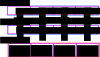
\includegraphics[width=0.8\textwidth]{mmx-mull.pdf}
    \end{center}
  \end{column}
  \begin{column}{0.5\textwidth}
    \begin{center}
    \texttt{PMULHW} - multiply store high\\ word of the result
    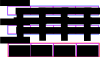
\includegraphics[width=0.8\textwidth]{mmx-mulh.pdf}
    \end{center}
  \end{column}
\end{columns}


\end{frame}


\begin{frame}[fragile]
\frametitle{MMX -- Example}

\begin{columns}[t,onlytextwidth]
  \begin{column}{0.5\textwidth}
Combine masked image with background:
\begin{lstlisting}[language={C},columns=flexible]
unsigned char mask[size],
 img1[size], img2[size];
if (mask[i]==0) {
  new_img[i] = img1[i];
} else {
  new_img[i] = img2[i];
}
\end{lstlisting}

  \end{column}
  \begin{column}{0.5\textwidth}
MMX implementation for 8 8-bit pixels in once
\begin{lstlisting}[language={[x86masm]Assembler},columns=flexible]
movq    mask_ptr, %mm0
pcmpeqb %mm0, 0
movq    %mm0, %mm1
pand    %mm1, obr1_ptr
pandn   %mm0, obr2_ptr
por     %mm0, %mm1
movq    %mm0, new_img_ptr
\end{lstlisting}
  \end{column}
\end{columns}
\end{frame}




\begin{frame}
\frametitle{3Dnow! Extension of MMX}
\begin{itemize}
\item The 3Dnow! extension added real number operations to the existing registers \texttt{mm0}-\texttt{mm7}.
\item Only allows pack two 32-bit/single real numbers in one register
\item Adds conversion of integers to real numbers and back, also using averaging of 8-bit and 16-bit integers
\item Addition, subtraction, multiplication, division of packed (pair of) real numbers
\item Comparing real numbers and finding minima and maxima

\end{itemize}
\end{frame}

\section{x86 SSE Extension}


\begin{frame}
\frametitle{x86 SSE Extension -- SIMD}
\begin{itemize}
\item SSE - Streaming SIMD Extension
\item new registers \texttt{xmm0}-\texttt{xmm7}
\item 128-bit wide each, next packed types can be used
\item $4\times$ float - 32-bit floating point number
\item $2\times$ double - 64-bit floating point number
\item extesion of MMX integer operations for 128-bit SSE registers
\end{itemize}
\end{frame}



\begin{frame}
\frametitle{x86 SSE Instructions}
\begin{itemize}

\item Operations: packed suffix -ps, scalar suffix -ss 



\item Load/store from/to memory: mov
\item Floating point math operations: add, sub, mul, div, rcp, sqrt, max, min, rsqrt
\item Logic operations on binary representation: and, or, xor, andn
\item Compare with mask set as the result: cmp, comi, ucomi


\item Scalar operations: addss, subss, mulss, divss
\end{itemize}
\end{frame}

\begin{frame}
\frametitle{x86 SSE Instructions on Packed Data}
\begin{columns}[t,onlytextwidth]
\begin{column}{0.5\textwidth}
\begin{center}
Packed operation

\includegraphics[width=0.9\textwidth]{sse.pdf}
\end{center}
\end{column}
\begin{column}{0.5\textwidth}
\begin{center}
Scalar operation

\includegraphics[width=0.9\textwidth]{sse-s.pdf}
\end{center}
\end{column}
\end{columns}
\end{frame}

\begin{frame}
\frametitle{Further x86 SSE Extensions}
Extension evolution in chronological order:
\begin{itemize}
\item SSE2 - 144 new instructions added
\item SSE3 - 13 yet additional intructions
\item SSSE3 - 16 additional intructions
\item SSE4 - 47 additional intructions
\item SSE4.2 - 170 additional intructions
\item AVX - Advanced Vector Extensions
\item AVX2 - widen to 256 bits (YMMx registers)
\item AVX-512 - 512 bits support (ZMMx registers)
\end{itemize}
\end{frame}


\end{document}

